\subsection{Similarity to the $g$-prior}
\label[misc]{misc:gprior}

The I-prior for $\boldsymbol{\beta}$ resembles the objective $g$-prior \citep{zellner1986assessing} for regression coefficients,
\[
  \boldsymbol{\beta} \sim \N_p\big(\bzero, g (\bX^\top \bPsi \bX)^{-1} \big),
\]
although they are quite different objects. 
The $g$-prior for $\boldsymbol{\beta}$ has the \emph{inverse} (scaled) Fisher information matrix as its covariance matrix.
This, in itself, has a much different and arguably counterintuitive meaning: large amounts of Fisher information about $\boldsymbol{\beta}$ corresponds to a small prior variance, and hence less deviation away from the prior mean of zero in estimating $\boldsymbol\beta$.
The choice of the hyperparameter $g$ has been the subject of much debate, with choices ranging from fixing $g=n$ (corresponding to the concept of \emph{unit Fisher information}), to fully Bayesian and empirical Bayesian methods of estimating $g$ from the data.

On the other hand, we note that the $g$-prior has an I-prior interpretation when argues as follows.
Assume that the regression function $f$ lies in the continual dual space of $\bbR^p$ equipped with the inner product $\ip{\bx,\bx'}_\cX = \bx^\top(\bX^\top \bPsi \bX)^{-1}\bx$.
With this inner product and from \cref{eq:fisher-linear-functional} (p. \labelcpageref{eq:fisher-linear-functional}), the Fisher information for $\boldsymbol{\beta}$ is
\begin{align*}
  \cI_g(\boldsymbol\beta) 
  &= \sum_{i=1}^n \sum_{j=1}^n \psi_{ij} (\bX^\top \bPsi \bX)^{-1}\bx_i \otimes (\bX^\top \bPsi \bX)^{-1}\bx_j \\
  &= (\bX^\top \bPsi \bX)^{-1} \cancel{(\bX^\top \bPsi \bX)} \cancel{(\bX^\top \bPsi \bX)^{-1}} \\
  &= (\bX^\top \bPsi \bX)^{-1},
\end{align*}
and this, rather than the usual $\bX^\top \bPsi \bX$ as the prior covariance matrix for $\boldsymbol{\beta}$, means that the I-prior is in fact the standard $g$-prior.

The metric induced by the inner product is actually the \emph{Mahalanobis distance}, a scale-invariant natural distance if the covariates are measured on different scales.
To expand on this idea, circle back to the regression function and write it as $f(\bx) = \ip{\bx,\boldsymbol\beta}_\cX$.
In usual least squares regression, the choice of inner product is irrelevant, so the usual dot product is commonly used (however, as we have seen above, the choice of inner product determines the form of the Fisher information for $\boldsymbol{\beta}$).
In particular, suppose that all the $x_{ik}$'s, $k=1,\dots,p$ for each unit $i=1,\dots,n$ are measured on the same scale; for instance, these could be measurements in centimetres.
In this case, the dot product is reasonable, because $\ip{\bx_i,\bx_j} = \sum_{k=1}^p x_{ik}x_{jk}$ and the inner product has a coherent unit, namely the squared unit of the $x_{ik}$'s.
However, if they were a mix of various scaled measurements, then obviously the inner product's unit is incoherent---one would be resorted to adding measurements in different units, for example, $\text{cm}^2$ and $\text{kg}^2$ and so on.
In such a case, a unitless inner product is appropriate, like the Mahalonobis inner product, which technically rescales the $x_{ik}$'s to unity.
In summary, if the covariates are all measured on the same scale, then the I-prior is appropriate, and if not, the $g$-prior is appropriate.

\subsection{Multilevel models}
\label[misc]{misc:multilevelmodels}

Write $\alpha=\beta_0$, and for simplicity, assume iid errors, i.e.,  $\bPsi = \psi\bI_n$.
The form of $f\in\cF$ is now $f(\bx_i^{(j)},j) = \sum_{i'=1}^{n_{j'}}\sum_{j'=1}^m h_\lambda\big((\bx_i^{(j)},j),(\bx_{i'}^{(j')},j')\big) w_{i'j'}$, where each $w_{i'j'}\sim\N(0,\psi^{-1})$.

%We have seen from the previous section that $f_1(\bx_i^{(j)}) = \tilde\bx_i^{(j)\top}\boldsymbol{\beta}$, with $\boldsymbol{\beta} = \lambda_1\tilde\bX^\top\bw \sim \N_p(\bzero, \lambda_1^2\psi \tilde\bX^\top\tilde\bX )$.
%Here, $\tilde\bX$ is the $(n_1+\cdots+n_m) \times p$ matrix containing centred entries $\tilde\bx_i^{(j)} := \bx_i^{(j)} - \frac{1}{n_j}\sum_{i=1}^{n_j}\bx_i^{(j)}$.
Now, functions in the scaled RKHS $\cF_2$ have the form
\begin{align*}
  f_2(j) 
  &= \sum_{i=1}^{n_{j'}}\sum_{j'=1}^m \lambda_2\left( \frac{\delta_{jj'}}{p_j} - 1 \right)w_{ij'} \\
  &=  \lambda_2\left( \frac{w_{+j}}{p_j} - w_{++} \right),
\end{align*}
where a `$+$' in the index of $w_{ik}$ indicates a summation over that index, and $p_j$ is the empirical distribution over $\cM$, i.e. $p_j = n_j/n$.
Clearly $f_2(j)$ is a variable depending on $j$, so write $f_2(j)=\beta_{0j}$.
The distribution of $\beta_{0j}$ is normal with zero mean and variance
\begin{align*}
  \Var \beta_{0j} 
  &= \lambda_2^2 \left( \frac{\cancel{n_j}\psi}{n_j^{\cancel{2}} / n^2} + n\psi \right)  \\
  &= n\psi\lambda_2^2 \left( \frac{1}{p_j} + 1 \right).
\end{align*}
The covariance between any two random intercepts $\beta_{0j}$ and $\beta_{0j'}$ is
\begin{align*}
  \Cov(\beta_{0j},\beta_{0j'})
  &= \Cov\left( \lambda_2\left( \frac{w_{+j}}{p_j} - w_{++} \right), \lambda_2\left( \frac{w_{+j'}}{p_{j'}} - w_{++} \right) \right)  \\
  &= \frac{\lambda_2^2}{p_j p_{j'}} \cancelto{0}{\Cov(w_{+j},w_{+j'})} - \frac{\lambda_2^2}{p_j} \Cov(w_{+j},w_{++}) - \frac{\lambda_2^2}{p_{j'}} \Cov(w_{++},w_{+j'}) \\
  &\phantom{==} + \lambda_2^2 \Cov(w_{++},w_{++}) \\
  &= - \frac{\lambda_2^2}{\cancel{n_j}/n} \cancel{n_j}\psi - \frac{\lambda_2^2}{\cancel{n_{j'}}/n} \cancel{n_{j'}}\psi + \lambda_2^2 n\psi \\
  &= -n\psi\lambda_2^2.
\end{align*}

Functions in $\cF_{12}$, on the other hand, have the form
\begin{align*}
  f_{12}(\bx_i, j)
  &= \sum_{i'=1}^{n_{j'}}\sum_{j'=1}^m \lambda_1\lambda_2 \cdot \tilde \bx_i^{(j)\top} \tilde \bx_{i'}^{(j')} \cdot \left( \frac{\delta_{jj'}}{p_j} - 1 \right)  w_{i'j'} \\
  &=  \tilde \bx_i^{(j)\top}   
  {\color{gray}
  \underbrace{\color{black}
  \left( \frac{\lambda_1\lambda_2}{p_j} \sum_{i'=1}^{n_{j}}  \tilde \bx_{i'}^{(j)} w_{i'j} - \lambda_1\lambda_2\sum_{i'=1}^{n_{j'}}\sum_{j'=1}^m  \tilde \bx_{i'}^{(j')}  w_{i'j'} \right)
  }_{\boldsymbol\beta_{1j}}},
\end{align*}
and this is, as expected, a linear form dependent on cluster $j$.
We can calculate the variance for $\beta_{1j}$ to be
\begin{align*}
  \Var \boldsymbol{\beta}_{1j}
  &= \lambda_1^2\lambda_2^2 \Var\left( \frac{1}{p_j} \tilde\bX_j^\top \bw_j - \tilde\bX^\top \bw \right) \\
  &= \lambda_1^2\lambda_2^2 \left( \frac{\psi}{n_j^2/n^2} \tilde\bX_j^\top\tilde\bX_j + \psi \tilde\bX^\top  \tilde\bX - \frac{1}{p_j} \tilde\bX_j^\top \Cov( \bw_j,\bw) \tilde\bX^\top  \right) \\
  &= n\psi\lambda_1^2\lambda_2^2 \left( \frac{1}{p_j}\bS_j +  \bS - \bS_{j} \right) \\
  &= n\psi\lambda_1^2\lambda_2^2 \left( \left(\frac{1}{p_j}-1\right)\bS_j +  \bS  \right)
\end{align*}
where $\bS_j = \frac{1}{n_j} \sum_{i=1}^{n_j} (\bx_i^{(j)} - \bar \bx)^\top(\bx_i^{(j)} - \bar \bx)$, $\bS = \frac{1}{n} \sum_{i=1}^{n_j} \sum_{j=1}^{m} (\bx_i^{(j)} -  \bar \bx)^\top(\bx_i^{(j)} - \bar \bx)$, and $\bar \bx = \frac{1}{n} \sum_{i=1}^{n_j} \sum_{j=1}^{m} \bx_i^{(j)}$.
The covariance between two vectors of the random slopes is
\begin{align*}
  \Cov(\boldsymbol{\beta}_{1j},\boldsymbol{\beta}_{1j'}) 
  &= \lambda_1^2\lambda_2^2  \Cov \left( \frac{1}{p_j} \tilde\bX_j^\top \bw_j - \tilde\bX^\top \bw, \frac{1}{p_{j'}} \tilde\bX_{j'}^\top \bw_{j'} - \tilde\bX^\top \bw  \right) \\
  &= \psi\lambda_1^2\lambda_2^2 \left( \tilde\bX^\top\tilde\bX - \frac{1}{p_j}\tilde\bX_j^\top\tilde\bX_j  - \frac{1}{p_{j'}}\tilde\bX_{j'}^\top\tilde\bX_{j'} \right) \\
  &= n\psi\lambda_1^2\lambda_2^2 \left( \bS - \bS_j - \bS_{j'}  \right).
\end{align*}

Another quantity of interest is the covariance between the random intercepts and random slopes:
\begin{align*}
  \Cov(\beta_{0j}, \boldsymbol{\beta}_{1j}) 
  &= \lambda_1\lambda_2^2  \Cov\left( \frac{1}{p_{j}} \bone_{n_j}^\top \bw_{j} - \bone_n^\top \bw, \frac{1}{p_{j}} \tilde\bX_{j}^\top \bw_{j} - \tilde\bX^\top \bw   \right) \\
  &= \psi\lambda_1\lambda_2^2  \left( \cancelto{0}{\bone_{n}^\top \tilde\bX} + \frac{1}{p_{j}^2} \bone_{n_j}^\top \tilde\bX_j  - \frac{2}{p_{j}} \bone_{n_{j}}^\top \tilde\bX_{j} \right) \\
  &= n\psi\lambda_1\lambda_2^2  \left(  \left(\frac{1}{p_j} - 2 \right) \frac{1}{n_{j}} \sum_{i=1}^{n_j}(\bx_i^{(j)} - \bar \bx)  \right) \\
  &= n\psi\lambda_1\lambda_2^2 \left(\frac{1}{p_j} - 2 \right) ( \bar\bx^{(j)}   -\bar \bx  ) 
\end{align*}
and
\begin{align*}
  \Cov(\beta_{0j}, \boldsymbol{\beta}_{1j'}) 
  &= \lambda_1\lambda_2^2  \Cov\left( \frac{1}{p_{j}} \bone_{n_j}^\top \bw_{j} - \bone_n^\top \bw, \frac{1}{p_{j'}} \tilde\bX_{j'}^\top \bw_{j'} - \tilde\bX^\top \bw   \right) \\
  &= \psi\lambda_1\lambda_2^2  \left( \cancelto{0}{\bone_{n}^\top \tilde\bX} + \frac{1}{p_{j}p_{j'}} \bone_{n_j}^\top \cancelto{0}{\Cov(\bw_j,\bw_{j'})} \tilde\bX_{j'} - \frac{1}{p_{j}} \bone_{n_j}^\top \tilde\bX_j  - \frac{1}{p_{j'}} \bone_{n_{j'}}^\top \tilde\bX_{j'} \right) \\
  &= n\psi\lambda_1\lambda_2^2  \left(  - \frac{1}{n_{j}} \sum_{i=1}^{n_j}(\bx_i^{(j)} - \bar \bx)  - \frac{1}{n_{j'}} \sum_{i=1}^{n_{j'}}(\bx_i^{(j')} - \bar \bx) \right) \\
  &= n\psi\lambda_1\lambda_2^2  \left(  2\bar \bx -  \bar\bx^{(j)}  -  \bar \bx^{(j')}  \right).
\end{align*}

\subsection{A recap on the exponential family EM algorithm}
\label{apx:expem}

Consider the density function $p(\cdot|\btheta)$ of the complete data $\bz = \{\by,\bw\}$, which depends on parameters $\btheta = (\theta_1,\dots,\theta_s)^\top \in\Theta\subseteq\bbR^s$, belonging to an exponential family of distributions.
This density takes the form $p(\bz|\btheta) = B(\bz) \exp \big( \ip{\bfeta(\btheta), \bT(\bz)} -  A(\btheta) \big)$, where $\bfeta:\bbR^s \mapsto \bbR$ is a link function,  $\bT(\bz) = \big(T_1(\bz),\dots,T_s(\bz)\big)^\top \in \bbR^s$ are the sufficient statistics of the distribution, and $\ip{\cdot,\cdot}$ is the usual Euclidean dot product.
It is often easier to work in the \emph{natural parameterisation} of the exponential family distribution
\begin{align}\label{eq:pdfexpfamnat}
  p(\bz|\bfeta) = B(\bz) \exp \big( \ip{\bfeta, \bT(\bz)} -  A^*(\bfeta) \big)
\end{align}
by defining $\bfeta := \big(\eta_1(\btheta),\dots,\eta_r(\btheta)\big) \in \cE$, and $\exp A^*(\bfeta) = \int B(\bz) \, \exp \, \ip{\bfeta, \bT(\bz)}  \dint \bz$ to ensure the density function normalises to one.
As an aside, the set $\cE := \big\{ \bfeta = (\eta_1,\dots,\eta_s) \,|\, \int  \exp A^*(\bfeta) < \infty \big\}$ is called the \emph{natural parameter space}.
If $\dim \cE = r < s = \dim \Theta$, then the the pdf belongs to the \emph{curved exponential family} of distributions.
If $\dim \cE = r = s = \dim \Theta$, then the family is a \emph{full exponential family}.

Assuming the latent $\bw$ variables are observed and working with the natural parameterisation, then the complete maximum likelihood (ML) estimate for $\bfeta$ is obtained by solving 
\begin{align}\label{eq:expEM1}
  \frac{\partial}{\partial\bfeta}\log p(\bz|\bfeta)
  &= \bT(\bz) - \frac{\partial}{\partial\bfeta} A^*(\bfeta) = 0.
\end{align}
Of course, the variable $\bw$ are never observed, so the ML estimate for $\bfeta$ can only be informed from what is observed.
Let $p(\by|\bfeta) = \int p(\by,\bw|\bfeta) \dint \bw$ represent the marginal density of the observations $\by$.
Now, the ML estimate for $\bfeta$  is obtained by solving
\begin{align}
  \frac{\partial}{\partial\bfeta}\log p(\by|\bfeta)
  &= \frac{1}{p(\by|\bfeta)} \cdot \frac{\partial}{\partial\bfeta}  p(\by|\bfeta) \nonumber \\
  &= \frac{1}{p(\by|\bfeta)} \cdot \frac{\partial}{\partial\bfeta} \left( \int p(\by,\bw|\bfeta) \dint \bw \right) \nonumber \\
  &= \frac{1}{p(\by|\bfeta)} \cdot \int \left( \frac{\partial}{\partial\bfeta} p(\by,\bw|\bfeta) \right) \dint \bw \nonumber \\
  &= \frac{1}{p(\by|\bfeta)} \cdot \int \left( p(\by,\bw|\bfeta) \frac{\partial}{\partial\bfeta} \log p(\by,\bw|\bfeta) \right) \dint \bw \nonumber \\
  &= \int \left( \bT(\by,\bw) - \frac{\partial}{\partial\bfeta} A^*(\bfeta) \right) p(\bw|\by,\bfeta) \dint \bw \nonumber \\
  &= \E_\bw \big[ \bT(\by,\bw) | \by \big] - \frac{\partial}{\partial\bfeta} A^*(\bfeta) \label{eq:expEM2}
\end{align}
equated to zero.
Note that we are allowed to change the order of integration and differentation provided the integrand is continuously differentiable.
So the only difference between the first order condition of \cref{eq:expEM1} and that of \cref{eq:expEM2} is that the sufficient statistics involving the unknown $\bw$ are replaced by their conditional or posterior expectations.
%but this is not an issue: by the law of total expectations, $\E\bT(\bz) = \E \bT(\by,\bw) = \E \big[ \E_\bw[\bT(\by,\bw)|\by] \big]$
%so solving $\bT(\bz) = \E \bT(\bz)$ for $\btheta$ is not possible without some manipulation.

A useful identity to know is that $\frac{\partial}{\partial\bfeta} A^*(\bfeta) = \E_\bz \bT(\bz)$ \citep[Theorem 3.4.2 \& Exercise 3.32(a)]{casella2002statistical}, which can be expressed in terms of the original parameters $\btheta$.
As a consequence, solving for the ML estimate for $\btheta$ from the FOC equations \cref{eq:expEM2} is possible without having to deal with the derivative of $A^*$ with respect to the natural parameters.
Having said this, an analytical solution in $\btheta$ may not exist, because the relationship of $\btheta$ could be implicit in the set of equations $\E_\bw \big[ \bT(\bw,\by) | \by, \btheta \big] = \E_{\by,\bw}\left[ \bT(\by,\bw) | \btheta \right]$.
One way around this is to employ an iterative procedure, as detailed in \cref{alg:EM3}.

\begin{algorithm}[hbt]
\caption{Exponential family EM}\label{alg:EM3}
\begin{algorithmic}[1]
  \State \textbf{initialise} $\btheta^{(0)}$ and $t\gets 0$
  \While{not converged}
    \State E-step: $\tilde\bT^{(t+1)}(\by,\bw) \gets \E_\bw \big[ \bT(\bw,\by) | \by, \btheta^{(t)} \big]$
    \State M-step: $\btheta^{(t+1)} \gets$ solution to $\tilde\bT^{(t+1)}(\by,\bw) = \E_{\by,\bw}\left[ \bT(\by,\bw) | \btheta \right]$
    \State $t \gets t + 1$
  \EndWhile
\end{algorithmic}
\end{algorithm}

To see how \cref{alg:EM3} motivates the EM algorithm, consider the following argument.
Recall that for the EM algorithm, the function $Q_t(\bfeta) = \E_\bw[\log p(\by,\bw|\bfeta) | \by,\bfeta^{(t)}]$ is maximised at each iteration $t$.
For exponential families of the form \cref{eq:pdfexpfamnat}, the $Q_t$ function turns out to be
\[
 Q_t(\bfeta) = \E_\bw \big[ \ip{\bfeta, \bT(\bz)} | \by,\bfeta^{(t)} \big] -  A^*(\bfeta) + \log B(\bz),
\]
and this is maximised at the value of $\bfeta$ satisfying
\begin{align*}
  \frac{\partial}{\partial\bfeta} Q_t(\bfeta)
  &= \E_\bw \big[ \bT(\by,\bw) | \by,\bfeta^{(t)} \big] - \frac{\partial}{\partial\bfeta}A^*(\bfeta) = 0,
\end{align*}
a similar condition to \cref{eq:expEM2} when obtaining ML estimate of $\bfeta$.
Thus, $Q_t$ is maximised by the solution to line 4 in Algorithm \cref{alg:EM3}.



%In other words, the ML estimate for $\btheta$ satisfies $\{ \btheta | \bT(\bz) = \E \bT(\bz) \} $
%Assume the inverse mapping $\bfeta^{-1}$ exists, then the ML estimates $\hat\btheta$ can be obtained as $\bfeta^{-1}(\hat\btheta)$ due to the invariance property of ML estimates.




\subsection{A brief introduction to Hamiltonian Monte Carlo}
\label[misc]{misc:hmc}

Hamiltonian Monte Carlo had its beginnings in statistical physics, with the \citeyear{duane1987hybrid} paper by \citeauthor{duane1987hybrid} using what they called `Hybrid Monte Carlo' in lattice models of quantum theory.
Their work merged the approaches of molecular dynamics and Markov chain Monte Carlo methods.
As interesting side note, their method abbreviates also to `HMC', but throughout the statistical literature, it is more commonly referred to by its more descriptive name Hamiltonian Monte Carlo.
Incidentally, the use of HMC started with applications to neural networks as early as 1996 (see \citet{neal2011mcmc} for an excellent review of the subject matter).
It was not until 2011 when active development of the method, and in particular, software for for statistical applications began.
The \proglang{Stan} initiative \citep{carpenter2016stan} began in response to difficulties faced when performing full Bayesian inference on multilevel generalised linear models.
These difficulties mainly involved poor efficiency in usual MCMC samplers, particularly high autocorrelations in the posterior chains, which meant that many chains and many iterations were required to get an adequate sample.
It was a case of exhausting all possible algorithmic remedies for existing samplers (Gibbs samplers, Metropolis samplers, etc.), and realising that fundamentally not much improvement can be had unless a novel sampling technique was discovered.

The basic idea behind HMC is to use Hamiltonian dynamics to propose new states in the posterior sampling, rather than relying on `random walks'.
If one were to understand and use the geometry of the posterior density to one's benefit, then it should be possible to generate new proposal states with high probabilities of acceptance and move far away from the current state.
Hamiltonian dynamics, like classical Newtonian mechanics, provides a framework for modelling the motion of a body in space across time $t$. 
Additionally, Hamiltonian dynamics concatenates the position vector $x$ with its momentum $z$, and the motion of $x$ in $d$-dimensional space is then described through Hamilton's equations
\begin{equation}\label{eq:hamilton1}
  \frac{\d x}{\d t} = \frac{\partial H}{\partial z}
  \hspace{0.5cm}\text{and}\hspace{0.5cm}
  \frac{\d z}{\d t} = -\frac{\partial H}{\partial x},
\end{equation}
where $H=H(x,z)$ is called the Hamiltonian of the system.
The Hamiltonian is an operator which encapsulates the total energy of the system.
In a closed system, one can express the sum of operators corresponding to the kinetic energy $K(p)$ and the potential energy $U(z)$ of the system
\begin{equation}\label{eq:hamilton2}
  H(x,z) = K(z) + U(x).
\end{equation}
Substituing \cref{eq:hamilton2} into \cref{eq:hamilton1}, we get the system of partial differential equations (PDEs)
\begin{equation}\label{eq:hamilton3}
  \frac{\d x}{\d t} = \frac{\partial}{\partial z} K(z)
  \hspace{0.5cm}\text{and}\hspace{0.5cm}
  \frac{\d z}{\d t} = -\frac{\partial}{\partial x}U(x).
\end{equation}

To describe the evolution of $\big(x(t),z(t)\big)$ from time $t$ to $t+T$, it is necessary to discretise time, and split $T = L\epsilon$.
The quantity $L$ is known as the number of \emph{leapfrogs}, and $\epsilon$ the \emph{step size}.
\begin{center}
  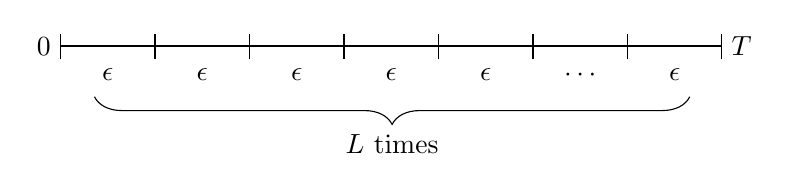
\begin{tikzpicture}[xscale=1.2, yscale=0.8]
    \draw [thick]  (0,0) -- (7,0);
    \foreach \x in  {0,1,2,3,4,5,6,7}
    \draw (\x,-.2) -- (\x, .2);
    \foreach \x in  {0.5,1.5,2.5,3.5,4.5}
    \node[align=center, below] at (\x,-.2) {$\epsilon$};
    \node[align=center, below] at (5.5,-.2) {$\cdots$};
    \node[align=center, below] at (6.5,-.2) {$\epsilon$};
    \node[align=center, left] at (0,0) {$0$};
    \node[align=center, right] at (7,0) {$T$};
    \draw[decorate, decoration={brace, mirror, amplitude=10pt}, xshift=-4pt, yshift=0pt]
    (0.5,-0.8) -- (6.8,-0.8) node [midway,below,yshift=-10pt] {$L$ times};
  \end{tikzpicture}
\end{center}
The system of PDEs is solved using Euler's method, or the more commonly used leapfrog integration, which is a three-step process:
\begin{table}[H]
  \centering
  \begin{tabular}{lrl}
    1. \textbf{Half-step momentum.} 
    &$z(t + \epsilon/2) =$ 
    &\hspace{-7pt}$z(t) - \frac{\epsilon}{2} \, \frac{\partial}{\partial x} U \big( x(t) \big)$ \\[0.6em]
    2. \textbf{Full-step position.} 
    &$x(t + \epsilon) =$ 
    &\hspace{-7pt}$x(t) + \epsilon \, \frac{\partial}{\partial  z} K \big(  z(t + \epsilon / 2) \big)$ \\[0.6em]
    3. \textbf{Half-step momentum.} 
    &$z(t + \epsilon) =$ 
    &\hspace{-7pt}$z(t + \epsilon/2) =  z(t) - \frac{\epsilon}{2} \, \frac{\partial}{\partial x} U \big( x(t) \big)$ \\[0.6em]
  \end{tabular}
\end{table}
\vspace{-1.5em}
\noindent in which steps 1--3 are repeated $L$ times.

Having knowing the formula for how particles move in space, we can use this information to treat random points drawn from some probability density as `particles'.
Randomness of position and momentum are prescribed through probability densities on each.
Given some energy function $E(\theta)$ over states $\theta$, the \emph{canonical distribution} of the states $\theta$ (otherwise known as the \emph{canonical ensemble}) is given by the probability density function
\[
  p(\theta) \propto \exp \left( -\frac{E(\theta)}{k\tau} \right),
\]
where $k$ is Boltzmann's constant, $\tau$ is the absolute temperature of the system.
The Hamiltonian is one such energy function over states $(x,z)$.
By replacing $E(\theta)$ by \cref{eq:hamilton2} in the pdf above, we realise that the distribution for $x$ and $z$ are independent.
The system can be manipulated such that $k\tau=1$---in any case, these are constants which can be absorbed into one of the terms in the pdf anyway.

Using a \emph{quadratic kinetic energy} function $K(z) = z^\top M^{-1} z/2$\footnotemark, we find that the probability density function for $z$ is
\[
  p(z) \propto \exp \left(-\half z^\top M^{-1} z \right),
\]
implying $z\sim\N_d(0,M)$.
Here, $M = \diag(m_1,\dots,m_d)$ is called the \emph{mass matrix}, which obviously serves as the variance for the randomly distributed $z$.
As for the potential energy, choose a function such that $U(x) = -\log p(x)$, implying $p(x) \propto \exp \big( -U(x) \big)$.
Here, $p(x)$ represents the target density from which we wish to sample, for instance, a posterior density of interest.
Thus, to sample variables $x$ from $p(x)$, one artificially introduces momentum variables $z$ and sample jointly instead from $p(x,z) = p(z)p(z)$, and discarding $z$ thereafter.
The HMC algorithm is summarised in \cref{alg:hmc}.

%\vspace{1em}
\algrenewcommand{\algorithmiccomment}[1]{{\color{gray} \hfill $\triangleright$ #1}}
\begin{algorithm}[hbt]
\caption{Hamiltonian Monte Carlo}
\label{alg:hmc}
\begin{algorithmic}[1]
  \State \textbf{initialise} $x^{(0)}$, $z^{(0)}$ and choose values for $L$, $\epsilon$ and $M$
  \While{not converged}
    \State Draw $z\sim\N_d(0,M)$ \Comment{Perturb momentum}
    \State Move $(x^{(t)},z^{(t)}) \mapsto (x^*,z^*)$ using Hamiltonian dynamics  \Comment{Proposal state}
    \State Accept/reject proposal state, i.e. \Comment{Metropolis update}
    \[
      (x^{(t+1)},z^{(t+1)}) \gets 
      \begin{cases}
        (x^*,z^*) & \text{w.p. } \min(1,A) \\
        (x^{(t)},z^{(t)}) & \text{otherwise}
      \end{cases}
    \]
    where
    \[
      A = \frac{p(x^*,z^*)}{(x^{(t)},z^{(t)})} = \exp\left( H(x,z) -  H(x^{(t)},z^{(t)}) \right)
    \]
  \EndWhile
  \State \textbf{return} Samples $\big\{x^{(t)} \,|\, t=1,2,\dots\big\}$
\end{algorithmic}
\end{algorithm}

\begin{figure}[p]
  \vspace{-10pt}
  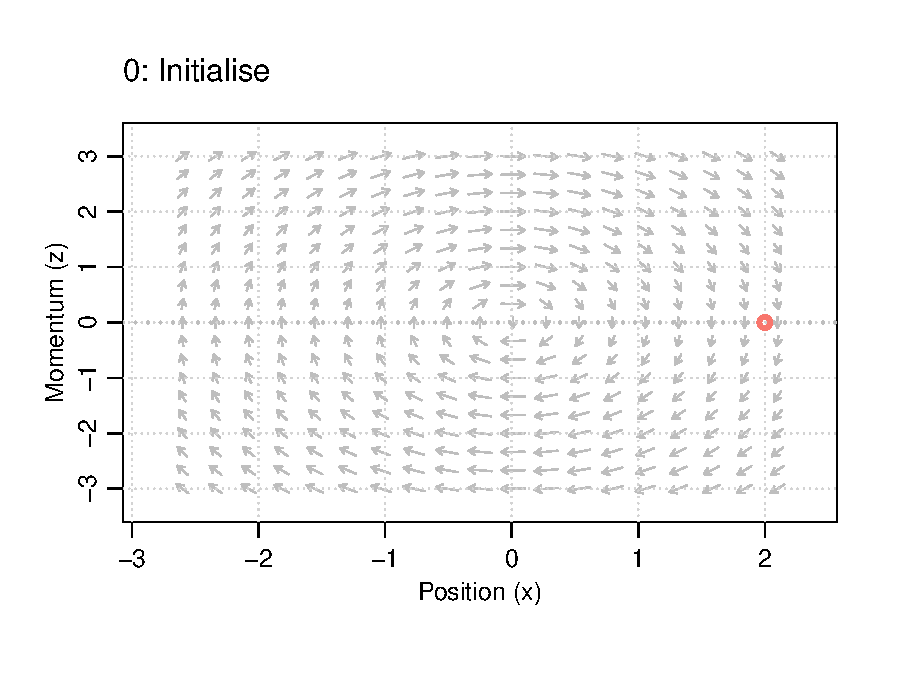
\includegraphics[width=0.49\textwidth]{figure/04-phase1}
  \vspace{-20pt}
  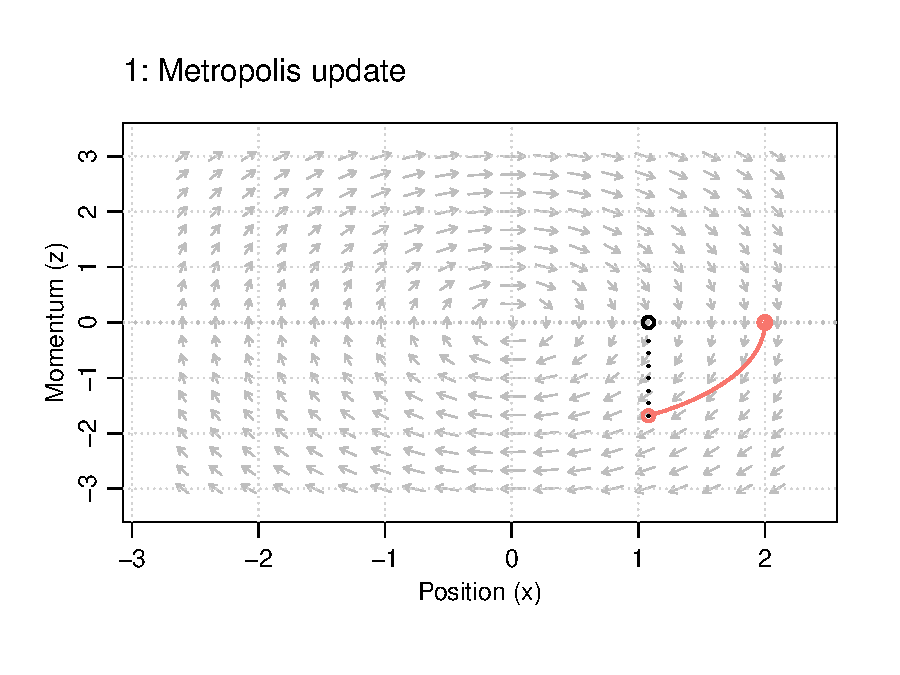
\includegraphics[width=0.49\textwidth]{figure/04-phase2}
  \vspace{-20pt}
  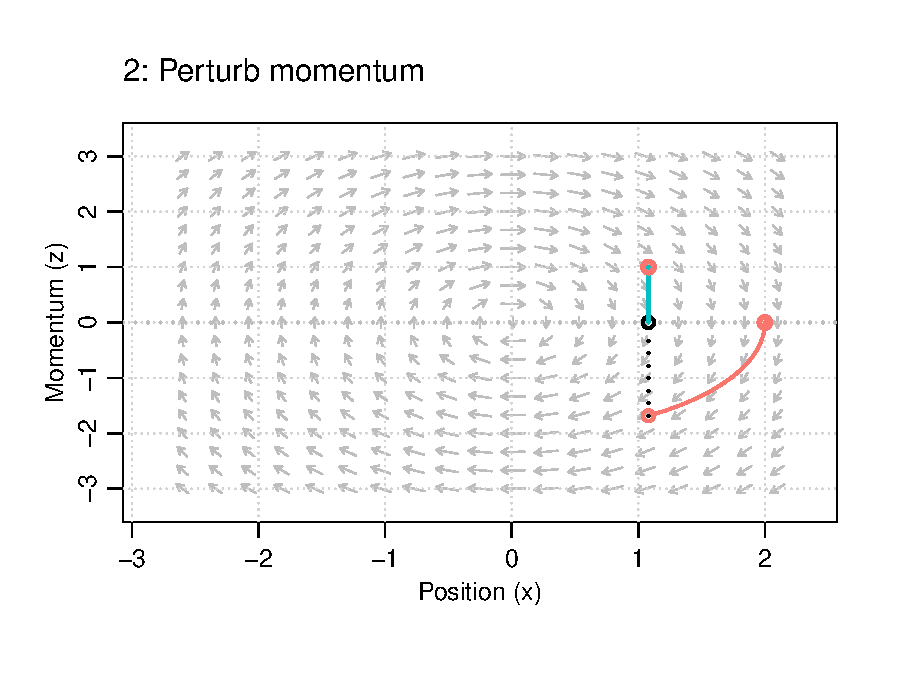
\includegraphics[width=0.49\textwidth]{figure/04-phase3}
  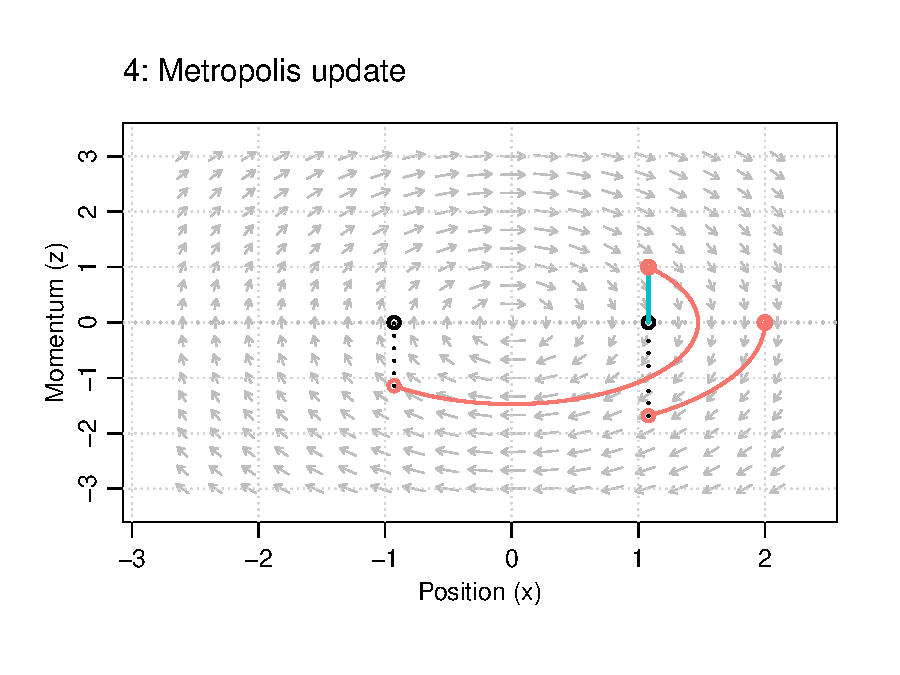
\includegraphics[width=0.49\textwidth]{figure/04-phase4}
  \vspace{-20pt}
  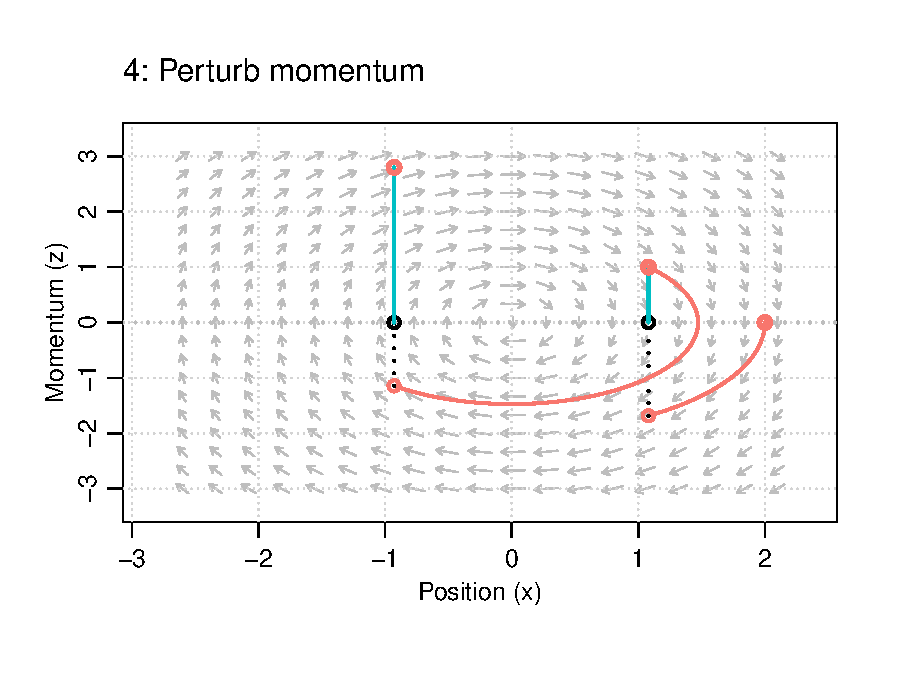
\includegraphics[width=0.49\textwidth]{figure/04-phase5}
  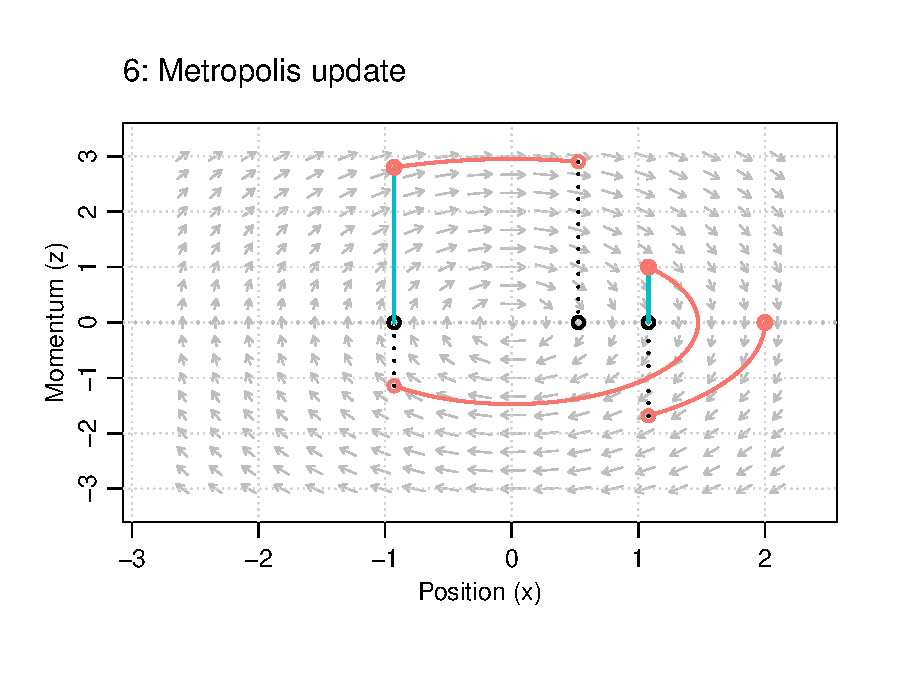
\includegraphics[width=0.49\textwidth]{figure/04-phase6}
  \vspace{-20pt}  
  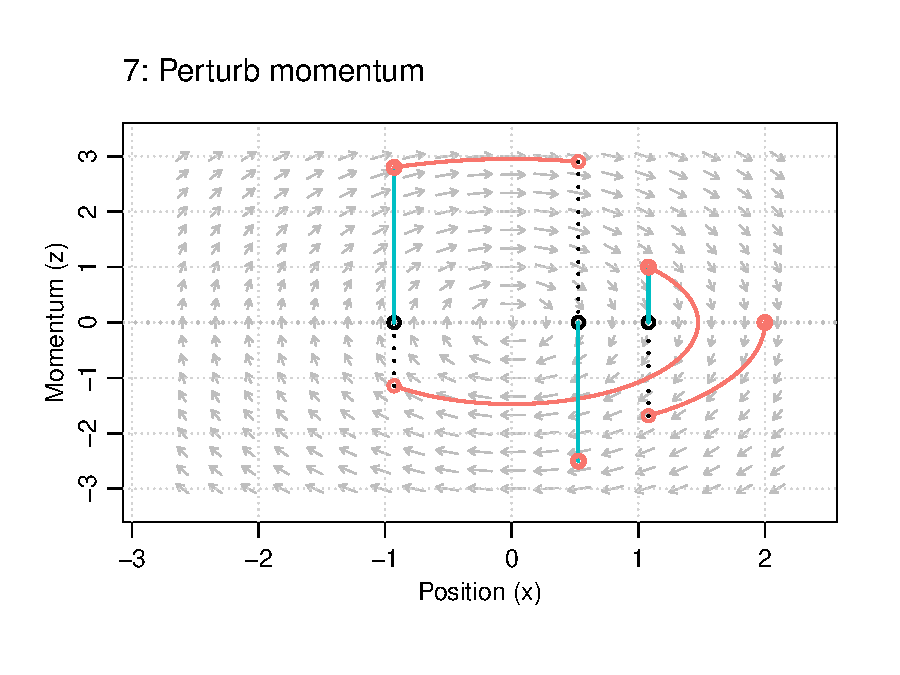
\includegraphics[width=0.49\textwidth]{figure/04-phase7}
  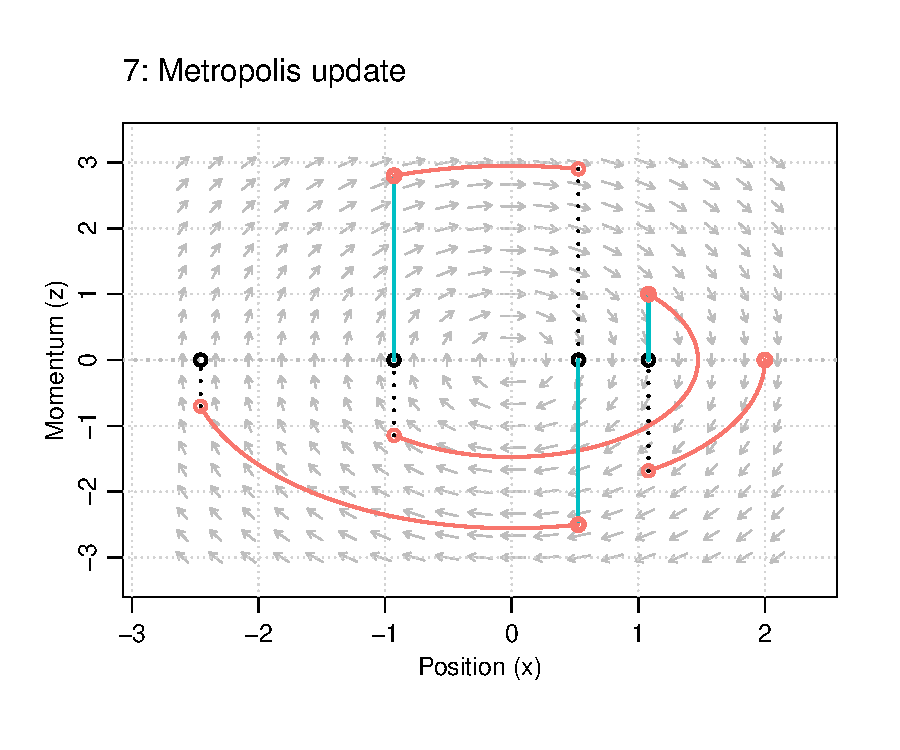
\includegraphics[width=0.49\textwidth]{figure/04-phase8}
  \caption{A phase diagram schematic of HMC sampling in one-dimension. At step 0, initialise values for momentum and position. At step 1, simulate movement using Hamiltonian dynamics, accept position and discard momentum. At step 2, perturb momentum using a normal density, then repeat.}
\end{figure}

HMC is often times superior to standard Gibbs sampling, for a variety of reasons. 
For one, conjugacy does not play any role in the efficiency of the HMC sampler, thus freeing the modeller to choose more appropriate and more intuitive prior densities for the parameters of the model. 
For another, the HMC sampler is designed to incite little autocorrelations between samples, and thus increasing efficiency.

Several drawbacks do exist with the HMC sampler. Firstly, it is impossible to directly sample from discrete distributions $p(x)$.
More concretely, HMC requires that the domain of $p(x)$ is continuous and that $\partial \log p(x) / \partial x$ is inexpensive to compute.
To work around this, one must reformulate the model by marginalising out the discrete variables, and obtain them back later by separately sampling from their posteriors.
Alternatively, a Gibbs sampler specifically for the discrete variables could be augmented with the HMC sampler.
The other drawback of HMC is that there are many tuning parameters (leapfrog $L$, step-size $\epsilon$, mass matrix $M$, etc.)  that is not immediately easy to perfect, at least not to the novice user. 

The implementation of HMC by the programming language \proglang{Stan}, which interfaces many other programming languages including \proglang{R}, \proglang{Python}, \proglang{MATLAB}, \proglang{Julia}, \proglang{Stata} and \proglang{Mathematica}, is a huge step forward in computational Bayesian analysis.
\proglang{Stan} takes the liberty of performing all the tuning necessary, and the practitioner is left with simply specifying the model. 
A vast library of differentiable probability functions are available, with the ability to bring your own code as well.
Development is very active and many improvements and optimisations have been made since its inception.

\footnotetext{Thinking back to elementary mechanics, this is the familiar $\half m v^2$ formula for kinetic energy and substituting in the identity $z =mv$, where $m$ is the mass of the object, and $v$ is its velocity.}
